\documentclass{article}
\usepackage{tikz,amsmath,amsthm,amssymb,tkz-graph,algpseudocode,booktabs,graphicx}
\usetikzlibrary{positioning}
\tikzset{box/.style={draw, thick, text centered, minimum height=0.5cm, minimum width=1cm}}
\tikzset{line/.style={draw, thick, -latex'}}
\graphicspath{{./images/}}
\title{CSC 226 Problem Set 4 Written Part}
\renewcommand{\thesubsection}{\thesection.\alph{subsection}}
\author{%
	Oliver Tonnesen\\
	V00885732}
\date{November 28, 2018}
\begin{document}
\maketitle
\section{Tragic Comedy and Network Flows}
We represend this problem with the following network graph:\\
Let $N(S)\equiv$number of people $p$ such that $p$ tolerates exactly $S$, $S\subseteq\{c_1,c_2,\ldots,c_k\}$.
\newline
\newline
\begin{figure}[h]
	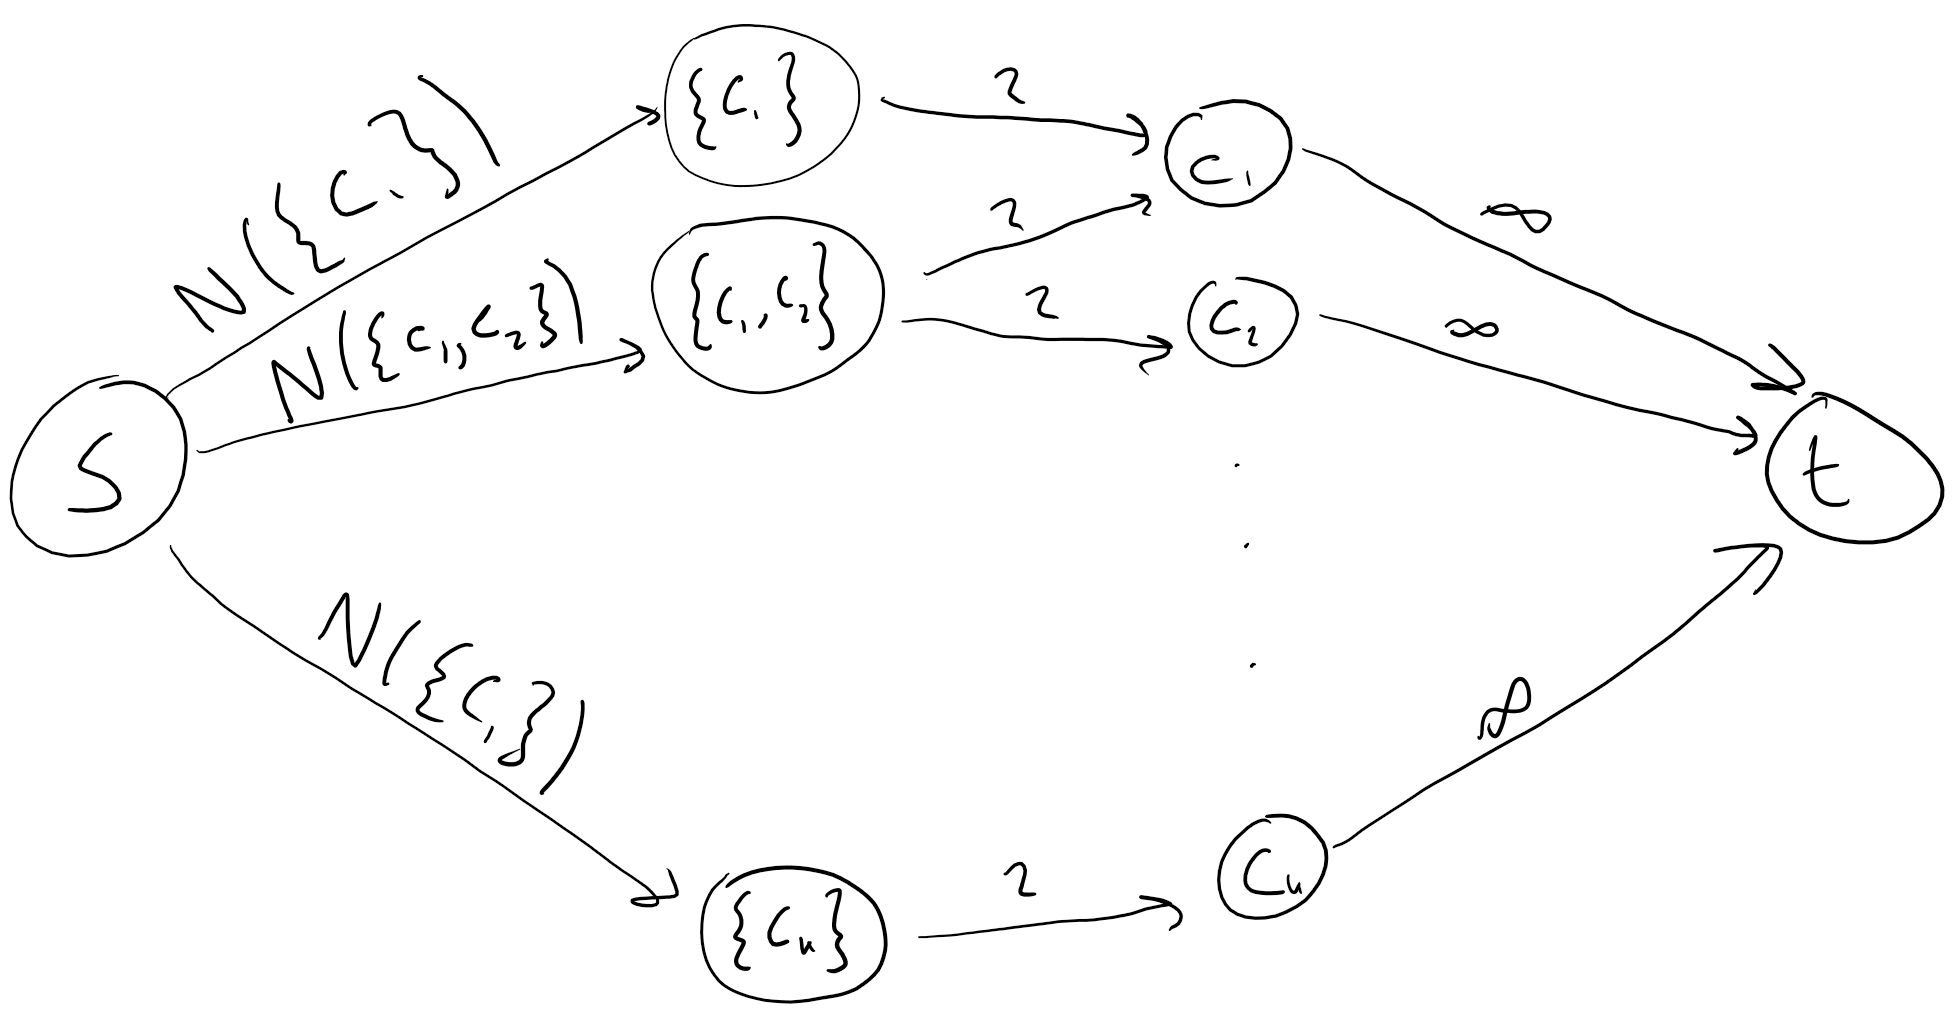
\includegraphics[scale=0.4]{NetGraph.png}
\end{figure}
\newline
\newline
Each comedian $c_i\in\{c_1,c_2,\ldots,c_j\}$ has a corresponding vertex $t_i$
in the network graph. Each subset $v_k\subseteq\{c_1,c_2,\ldots,c_j\}$ has a
corresponding vertex $n_k$ such that $n_k$ flows to $t_i$ if and only if
$c_i\in V_k$. Every passenger $p_l$ represents the one unit of flow from the
source vertex to the vertex $n_k$ such that the subset of comedians that $p_l$
will tolerate is equal to $v_k$.
\newline
\newline
If we restrict the capacity of the flow from any $n_k$ to any $n_k$ to 2, then
this network graph fully represents the given problem. If we now apply an
algorithm to this graph to determine its maximum flow, we will have efficiently
answered the question of whether or not it is possible to evacuate everyone
onboard.
\section{Max-Flow with Node Capacities}
\begin{tikzpicture}
\end{tikzpicture}
We can simply construct a standard network graph given such a node-capacited
network. The Ford-Fulkerson algorithm can then be applied directly. We
construct the network graph as follows:\\
For every vertex in the graph -- starting from the sink -- do the following:\\
Let each edge flowing to it have the nodes capacity. Let every edge flowing
from it have capacity equal to
$\min(\text{edge's currenct capacity},\text{node's capacity})$. Perform this
process recursively until each edge has a capacity.\\\\
This transformation takes $O(n+m)$ operations. Note that the Ford-Fulkerson
algorithm takes $O(m|f^*|)$ operations, where $f^*$ is the maximum flow in the
network. We know $m\ge n-1$, so $n+m\in O(m|f^*|)$, and our transformation does
not change the asymptotic running time of the solution.
\section{Min-cut and increasing all edge capacities by 1}
Suppose $(A^*,B^*)$ is no longer a minimum cut after the transformation. Then
there must exist some $(A',B')$ such that:
\begin{align}
	\sum_{a\in A^*}\sum_{b\in B^*} f(a,b)-\sum_{a\in A^*}\sum_{b\in B^*} f(b,a)\le
	\sum_{a\in A'}\sum_{b\in B'} f(a,b)-\sum_{a\in A'}\sum_{b\in B'} f(b,a)
\end{align}
and
\begin{align}
	\sum_{a\in A^*}\sum_{b\in B^*} [f(a,b)+1]-\sum_{a\in A^*}\sum_{b\in B^*} [f(b,a)+1]>
	\sum_{a\in A'}\sum_{b\in B'} [f(a,b)+1]-\sum_{a\in A'}\sum_{b\in B'} [f(b,a)+1]
\end{align}
\begin{align*}
	&\sum_{a\in A^*}\sum_{b\in B^*} [f(a,b)+1]-\sum_{a\in A^*}\sum_{b\in B^*} [f(b,a)+1]\\
	&=\Bigg[\sum_{a\in A^*}\sum_{b\in B^*} f(a,b) + \sum_{a\in A^*}\sum_{b\in B^*} 1\Bigg]
	-\Bigg[\sum_{a\in A^*}\sum_{b\in B^*} f(b,a) + \sum_{a\in A^*}\sum_{b\in B^*} 1\Bigg]\\
	&=\sum_{a\in A^*}\sum_{b\in B^*} f(a,b) - \sum_{a\in A^*}\sum_{b\in B^*} f(b,a)\\\\
	&\sum_{a\in A'}\sum_{b\in B'} [f(a,b)+1]-\sum_{a\in A'}\sum_{b\in B'} [f(b,a)+1]\\
	&=\Bigg[\sum_{a\in A'}\sum_{b\in B'} f(a,b) + \sum_{a\in A'}\sum_{b\in B'} 1\Bigg]
	-\Bigg[\sum_{a\in A'}\sum_{b\in B'} f(b,a) + \sum_{a\in A'}\sum_{b\in B'} 1\Bigg]\\
	&=\sum_{a\in A'}\sum_{b\in B'} f(a,b) - \sum_{a\in A'}\sum_{b\in B'} f(b,a)
\end{align*}
So clearly (1) and (2) cannot both be correct, and therefore no such cut
$(A',B')$ exists.\hfill\ensuremath{\square}
\section{Knuth-Morris-Pratt}
\begin{minipage}{.5\textwidth}
\begin{center}
	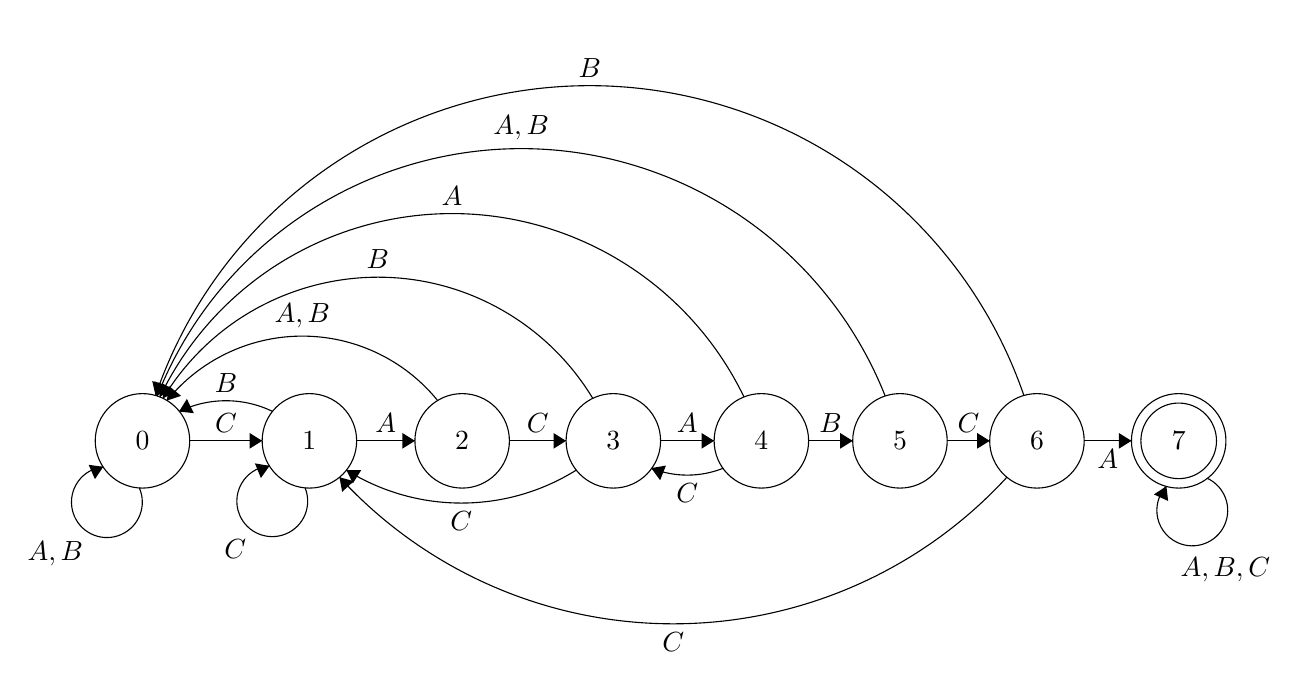
\begin{tikzpicture}[scale=0.2]
		\tikzstyle{every node}+=[inner sep=0pt]
		\draw [black] (73.4,-29.2) circle (3);
		\draw (73.4,-29.2) node {$7$};
		\draw [black] (73.4,-29.2) circle (2.4);
		\draw [black] (27.9,-29.2) circle (3);
		\draw (27.9,-29.2) node {$2$};
		\draw [black] (37.5,-29.2) circle (3);
		\draw (37.5,-29.2) node {$3$};
		\draw [black] (46.9,-29.2) circle (3);
		\draw (46.9,-29.2) node {$4$};
		\draw [black] (55.7,-29.2) circle (3);
		\draw (55.7,-29.2) node {$5$};
		\draw [black] (64.4,-29.2) circle (3);
		\draw (64.4,-29.2) node {$6$};
		\draw [black] (7.6,-29.2) circle (3);
		\draw (7.6,-29.2) node {$0$};
		\draw [black] (18.2,-29.2) circle (3);
		\draw (18.2,-29.2) node {$1$};
		\draw [black] (10.6,-29.2) -- (15.2,-29.2);
		\fill [black] (15.2,-29.2) -- (14.4,-28.7) -- (14.4,-29.7);
		\draw (12.9,-28.7) node [above] {$C$};
		\draw [black] (21.2,-29.2) -- (24.9,-29.2);
		\fill [black] (24.9,-29.2) -- (24.1,-28.7) -- (24.1,-29.7);
		\draw (23.05,-28.7) node [above] {$A$};
		\draw [black] (30.9,-29.2) -- (34.5,-29.2);
		\fill [black] (34.5,-29.2) -- (33.7,-28.7) -- (33.7,-29.7);
		\draw (32.7,-28.7) node [above] {$C$};
		\draw [black] (40.5,-29.2) -- (43.9,-29.2);
		\fill [black] (43.9,-29.2) -- (43.1,-28.7) -- (43.1,-29.7);
		\draw (42.2,-28.7) node [above] {$A$};
		\draw [black] (49.9,-29.2) -- (52.7,-29.2);
		\fill [black] (52.7,-29.2) -- (51.9,-28.7) -- (51.9,-29.7);
		\draw (51.3,-28.7) node [above] {$B$};
		\draw [black] (58.7,-29.2) -- (61.4,-29.2);
		\fill [black] (61.4,-29.2) -- (60.6,-28.7) -- (60.6,-29.7);
		\draw (60.05,-28.7) node [above] {$C$};
		\draw [black] (67.4,-29.2) -- (70.4,-29.2);
		\fill [black] (70.4,-29.2) -- (69.6,-28.7) -- (69.6,-29.7);
		\draw (68.9,-29.7) node [below] {$A$};
		\draw [black] (7.397,-32.181) arc (23.84511:-264.15489:2.25);
		\draw (2.07,-35.54) node [below] {$A,B$};
		\fill [black] (5.11,-30.85) -- (4.18,-30.72) -- (4.58,-31.63);
		\draw [black] (9.922,-27.34) arc (116.02993:63.97007:6.785);
		\fill [black] (9.92,-27.34) -- (10.86,-27.44) -- (10.42,-26.54);
		\draw (12.9,-26.15) node [above] {$B$};
		\draw [black] (17.921,-32.175) arc (22.3786:-265.6214:2.25);
		\draw (13.49,-35.45) node [below] {$C$};
		\fill [black] (15.67,-30.79) -- (14.74,-30.63) -- (15.12,-31.56);
		\draw [black] (9.153,-26.644) arc (140.94941:39.05059:11.07);
		\fill [black] (9.15,-26.64) -- (10.05,-26.34) -- (9.27,-25.71);
		\draw (17.75,-22.05) node [above] {$A,B$};
		\draw [black] (8.903,-26.503) arc (148.82631:31.17369:15.95);
		\fill [black] (8.9,-26.5) -- (9.74,-26.08) -- (8.89,-25.56);
		\draw (22.55,-18.31) node [above] {$B$};
		\draw [black] (35.15,-31.055) arc (-57.96047:-122.03953:13.76);
		\fill [black] (20.55,-31.06) -- (20.96,-31.9) -- (21.49,-31.06);
		\draw (27.85,-33.65) node [below] {$C$};
		\draw [black] (8.703,-26.413) arc (154.23039:25.76961:20.595);
		\fill [black] (8.7,-26.41) -- (9.5,-25.91) -- (8.6,-25.48);
		\draw (27.25,-14.27) node [above] {$A$};
		\draw [black] (44.489,-30.935) arc (-68.2056:-111.7944:6.165);
		\fill [black] (39.91,-30.93) -- (40.47,-31.7) -- (40.84,-30.77);
		\draw (42.2,-31.88) node [below] {$C$};
		\draw [black] (8.535,-26.351) arc (158.37563:21.62437:24.865);
		\fill [black] (8.53,-26.35) -- (9.29,-25.79) -- (8.36,-25.42);
		\draw (31.65,-10.15) node [above] {$A,B$};
		\draw [black] (62.489,-31.511) arc (-42.5738:-137.4262:28.774);
		\fill [black] (20.11,-31.51) -- (20.28,-32.44) -- (21.02,-31.76);
		\draw (41.3,-41.32) node [below] {$C$};
		\draw [black] (8.429,-26.318) arc (160.99752:19.00248:29.16);
		\fill [black] (8.43,-26.32) -- (9.16,-25.72) -- (8.22,-25.4);
		\draw (36,-6.15) node [above] {$B$};
		\draw [black] (75.212,-31.576) arc (65.05454:-222.94546:2.25);
		\draw (76.36,-36.6) node [below] {$A,B,C$};
		\fill [black] (72.62,-32.08) -- (71.83,-32.6) -- (72.73,-33.02);
	\end{tikzpicture}
\end{center}

\end{minipage}
\begin{center}
	\begin{tabular}{c|cccccccc}
		&0&1&2&3&4&5&6&7 \\
		\toprule
		A&0&2&0&4&0&0&7&7 \\
		B&0&0&0&0&5&0&0&7 \\
		C&1&1&3&1&3&6&1&7 \\
		\bottomrule
	\end{tabular}
\end{center}
\section{Rabin-Karp and Wildcards}
Since we know at which index the wildcard occurs, we can simply modify the hash
function to disregard whatever character falls on that index when computing the hash value.
\end{document}
